\section{Verlustbehaftete Kompression von volumetrischen Punkten}\label{einleitung}
Moderne Simulationen sind in der Lage grosse Mengen an Daten zu produzieren. Die rohe Datenmenge ist oft zu gross um sie zu archivieren oder in vernünftiger Zeit über eine Internetverbindung zu übertragen. In wissenschaftlichen Simulationen werden natürliche Phänomene wie Schwingungen, Flugbahnen, Kraftfelder etc. als Menge von Kurven im dreidimensionalen Raum abgebildet. Die Kurven sind dargestellt als Folge von Punkten. Ziel dieser Arbeit ist es eine verlustbehaftete Kompression für die Punktfolgen zu entwickeln, welche die Übertragung über eine Internetverbindung ermöglicht.

Im Rahmen dieses Projekts sollen Daten von Magnetfeldlinien der Sonne komprimiert werden, welche über eine Internetverbindung zum JHelioviewer übertragen werden. Der JHelioviewer ist eine Applikation zur visualisierung von Satellitenmessdaten und Simulationen der Sonne. Die Applikation wird von der ESA und der FHNW entwickelt. Die Abbildung \ref{einleitung::feldlinien} zeigt eine Visualisierung des JHelioviewers von der Sonnenoberfläche und Feldlinien.\\
\begin{figure}[!htbp]
\center
	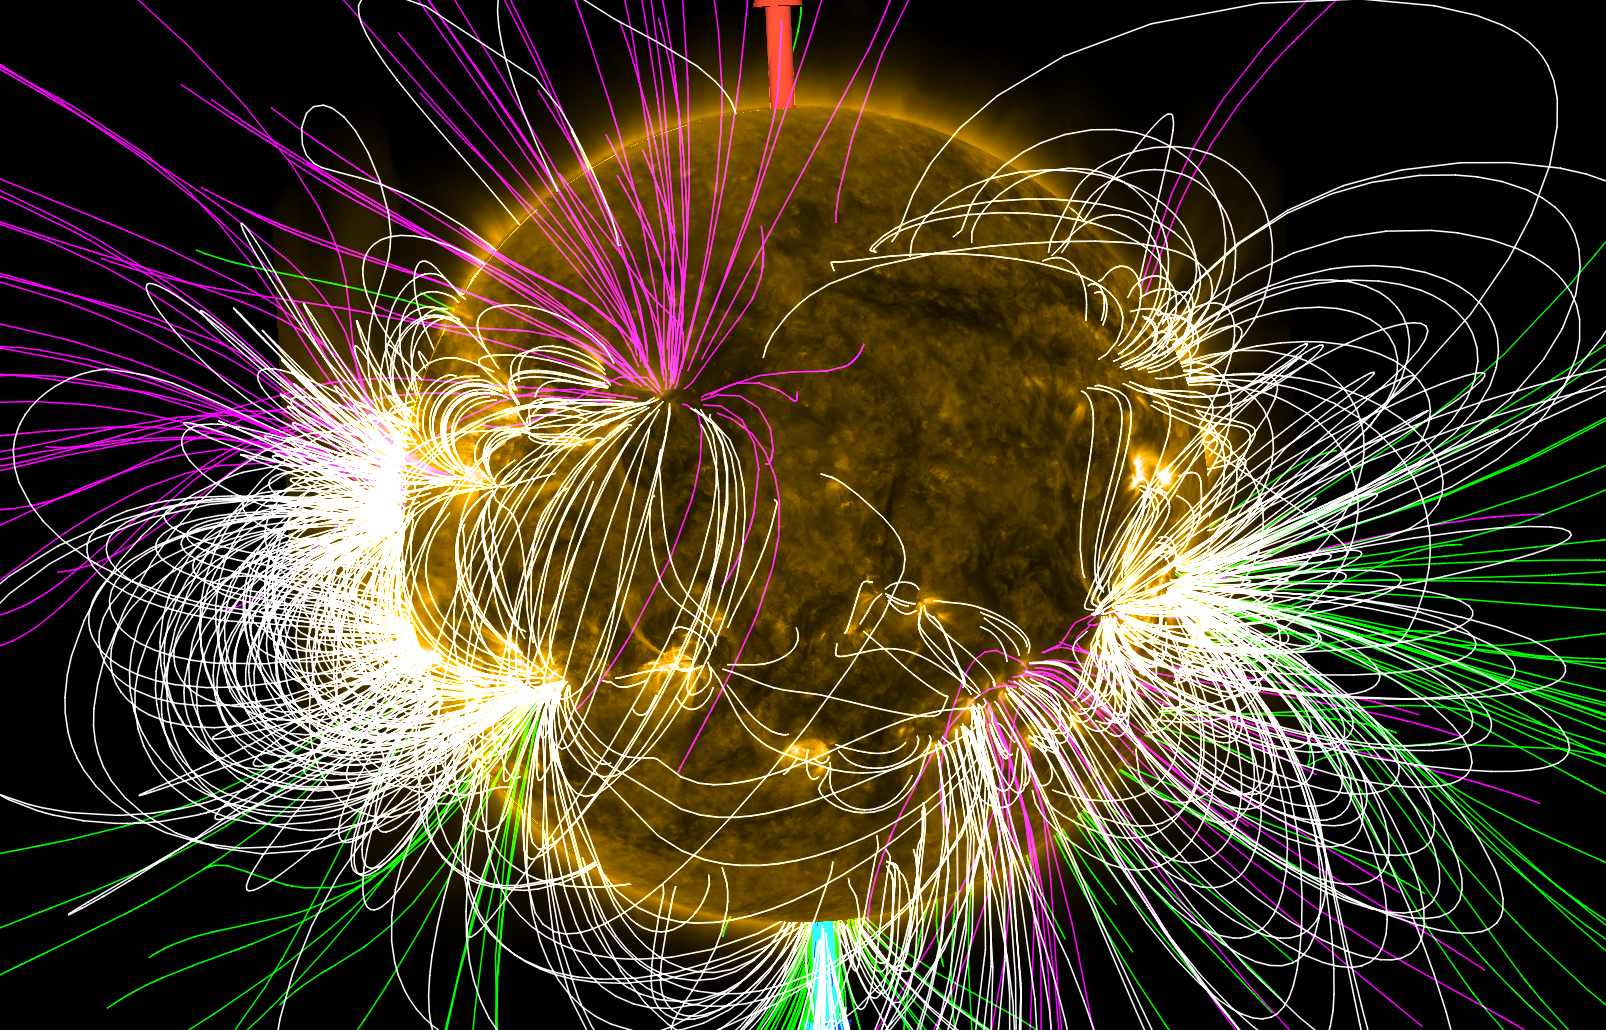
\includegraphics[width=0.8\textwidth,height=8cm,keepaspectratio]{./pictures/einleitung/fieldLines.png}
	\caption{Visualisierung der Feldlinien im JHelioviewer}
	\label{einleitung::feldlinien}
\end{figure}
Auf der Visualisierung sind Feldlinien in drei unterschiedlichen Farben zu erkennen, welche drei unterschiedle Typen darstellen: Linien, die auf der Sonne starten und wieder auf der Sonne landen, auf der Sonne starten und ins Weltall führen oder vom Weltall auf der Sonne landen. Die weissen Feldlinien repräsentieren ''Sonne zu Sonne´´, die Grünen ''Sonne zu Weltall´´ und die Violetten ''Weltall zu Sonne´´.

Im Vorfeld wurde bereits eine verlustbehaftete Kompression entwickelt, welche die Datenmenge auf durchschnittlich 1 Megabyte pro Simulation reduziert. Der JHelioviewer erstellt eine Animation der unterschiedlichen Daten, so werden nicht eine sondern mehrere Simulationen in Abfolge visualisiert. Es soll möglich sein, 1000 komprimierte Simulationen zwischenzuspeichern und möglichst wenig Arbeitsspeicher in Anspruch zu nehmen. In erster Linie wird erforscht, wie eine Kompression das Caching realisierbar macht. Ziel ist es eine Kompressionsrate von 8 bis 10 zu erreichen mit einer vergleichbaren Qualität zur Ist-Kompression.\\
Dass der Benutzer nicht immer warten muss, bis alle Simulationen heruntergeladen wurden, wird in dieser Arbeit nach Streamingmöglichkeiten gesucht.

Die Feldlinien werden mit einer Potential Field Source Surface (PFSS) Simulation berechnet, welche aus Messungen der Sonnenoberfläche die Feldlinien extrapoliert. Pro Simulation werden ungefähr 1.5 Mibyte an Daten produziert. Über eine Internetverbindung stellt ein Server die Simulationsdaten bereit.\\
Der JHelioviewer visualisiert eine Abfolge von Messungen und Simulationen, welche zur Laufzeit über eine Internetverbindung geladen werden. Für die Visualisierung der Feldlinien bedeutet das, dass mehrere Simulationen geladen werden müssen und dass die Bandbreite von anderen Daten bereits beansprucht wird. Deshalb soll eine verlustbehaftete Kompression umgesetzt werden, welche das Übertragen der Simulationen beschleunigt und weniger Bandbreitenintensiv gestaltet.\\
[\baselineskip]
Im laufe des Projekts wurden zwei Kompressionen entwickelt. Die Kompressionsraten sind der Tabelle \ref{einleitung:tabelle} ersichtlich.
\begin{table}[!htbp]
	\center
	\begin{tabular}{r|l}
		Lösungsansatz & Kompressionsraten \\\hline
		Ist-Zustand & 1\\
		Adaptives Subsampling & 11.6 \\
		Diskrete Kosinus Transformation & 14.1 \\
	\end{tabular}
	\caption{Tabelle der Lösungsansätzen und dessen Kompressionsraten.}
	\label{einleitung:tabelle}
\end{table}
